\begin{frame}
	\begin{center}
		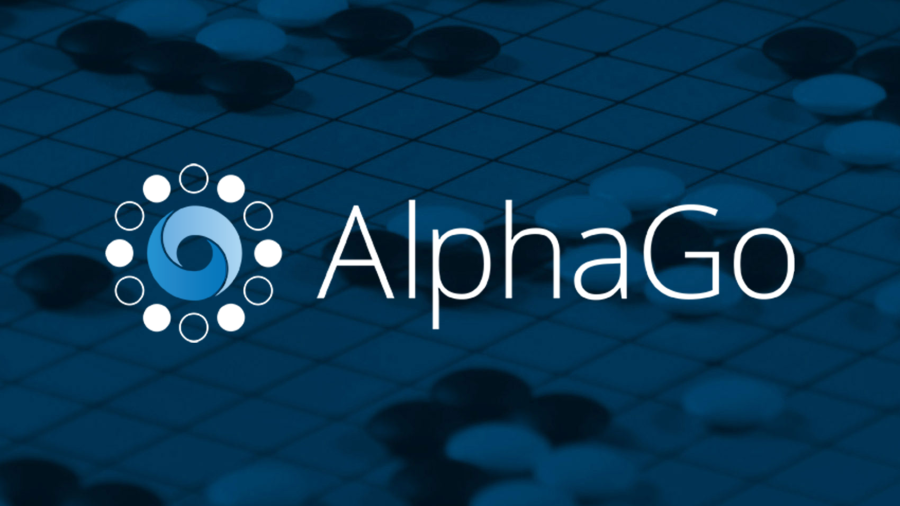
\includegraphics[width=8cm]{ressources/AlphaGoLogo}

	\end{center}
\end{frame}


\begin{frame}{AlphaGo}
	\begin{itemize}
		\item Développé par Google DeepMind
		\item En mars 2016 \textbf{AlphaGo} a battu Lee Sedol, l'un des meilleurs joueurs de Go
		\item Technologies utilisées:
		      \begin{itemize}
			      \item Apprentissage par renforcement
			      \item Réseaux de neurones profonds
			      \item Monte Carlo Tree Search
		      \end{itemize}
	\end{itemize}
\end{frame}



\begin{frame}{AlphaGo}{Composants}
	\begin{columns}[t]
		\begin{column}{.3\textwidth}
			\begin{block}{Rollout policy}
				Politique plus simple que les autres qui permet une simulation rapide du reste de la partie. Elle est amplement utilisée dans la simulation du MCTS.
			\end{block}
		\end{column}
		\begin{column}{.3\textwidth}
			\begin{block}{Policy network}
				Réseau neuronal qui renvoie une distribution de probabilité sur le coups possibles.
			\end{block}
		\end{column}
		\begin{column}{.3\textwidth}
			\begin{block}{Value Network}
				Réseau neuronal chargé de estimer la valuer d'une position, c'est-à-dire, les possibilité de gagner.
			\end{block}
		\end{column}
	\end{columns}
\end{frame}

\begin{frame}{AlphaGo}{Entraînement des Réseaux neuronales}
	\begin{center}
		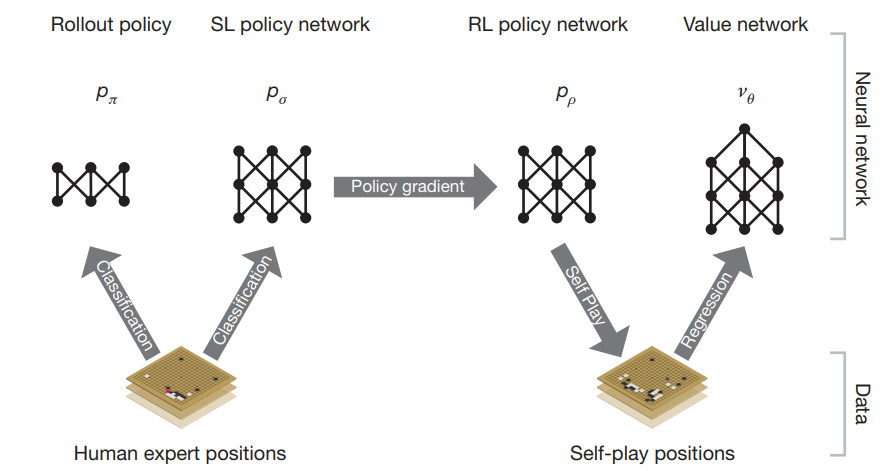
\includegraphics[width=7cm]{ressources/Entrainement}
		\begin{columns}[t]
			\begin{column}{.4\textwidth}
				\begin{block}{Avec un modèle}
					Entrainement d'un réseaux supervisé (SL) avec 30 millions de positions.
				\end{block}
			\end{column}
			\begin{column}{.4\textwidth}
				\begin{block}{Self-play}
					Apprentisage par renforcement à partir du SL en jouant des parties contre soi-même.
				\end{block}
			\end{column}
		\end{columns}

	\end{center}

\end{frame}


\begin{frame}{AlphaGo}{Apprentissage avec un modèle (SL)}

	\begin{itemize}
		\item Entraînement initial supervisé à partir de parties jouées par des professionnels (30 million de positions différentes)
		\item Le modèle doit prédire, à partir d'un état, le coup qu'un humain aurait fait
	\end{itemize}

\end{frame}


\begin{frame}{AlphaGo}{Self-play}

	\begin{itemize}
		\item Parties entre la version actuelle de l'agent et une version antérieure aléatoire
		\item Système de recompense simple : +1 si victoire et -1 si défaite
	\end{itemize}

\end{frame}


\begin{frame}{AlphaGo}{Velue network}
	\begin{itemize}
		\item Réseau neuronal qui permet d'évaluer la \textit{qualité} d'une position.
		\item Il est entraîné à partir de la policy network.
		\item
	\end{itemize}
\end{frame}


\begin{frame}{MCTS}

\end{frame}
